\documentclass[a4paper,13pt]{report}
\usepackage{polski}
\usepackage[utf8]{inputenc}
\usepackage[margin=1in,left=1.5in,includefoot]{geometry}
\usepackage{fancyhdr}
\usepackage{wrapfig}

\pagestyle{fancy}
\usepackage{graphicx}

\graphicspath{ {./images/} }

\begin{document}

\begin{titlepage}

\title{Praca inżynierska}
\author{Kamil Susek}
\date{September 2020}

\maketitle
\end{titlepage}
\chapter{Wprowadzenie}



\newpage

\chapter{Wstępna analiza dziedziny.}
Elektroniczne systemy głosowania coraz bardziej zyskują na popularności.
Wraz z postępem technologii oraz coraz większego znaczenia internetu w życiu 
społecznym, pojawiają się pomysły (a nawet implementacje) przeniesienia procesu głosowania do sieci. Pomysły i implementacje internetowych systemów wyborczych dotyczą wyborów na szczeblu państwowym (przykładowo wybory prezydenckie), jak i wyborów organizowanych na potrzeby prywatne. System e-votingu zazwyczaj sprowadza się do serwisu internetowego, który pozwala na oddanie głosu poprzez odpowiednią stronę internetową. 

Przeniesienie głosowania do aplikacji internetowej, pozwala zminimalizować wpływ ewentualnego błędu ludzkiego podczas przeprowadzania wyborów. Jednakże takie rozwiązanie generuje nowe problemy, z którymi muszą się zmierzyć projektanci tych systemów. Największy problem stanowi zabezpieczenie aplikacji, przed zewnętrznymi próbami fałszowania wyników głosowania. Rozwój technologii prowadzi również do powstawania nowych odmian “złośliwego oprogramowania”, co prowadzi do ciągłego aktualizowania zabezpieczeń. Aplikacja odpowiadająca na potrzeby wyborów, na wysokim szczeblu powinna być tworzona “na potrzeby danych czasów”, bądź łatwa w płynnej aktualizacji.

Zabezpieczenie przed fałszowaniem głosów to nie jest jedyny problem, z jakim trzeba się zmierzyć podczas próby przeniesienia procesu głosowania do internetu. Kolejnym problemem jest sama logika systemu głosowania, niektóre wybory wymagają, aby informacje o wyborcach oraz ich głosach, były tajne. System powinien również umożliwiać weryfikację użytkownika, na podstawie dostarczonych przez organizatora wyborów danych logowania. Coraz głębsza analiza problemu generuje coraz więcej potrzeb z zakresu bezpieczeństwa systemu. Dodatkowo wyszczególniając elementy, które powinny podlegać szczególnej protekcji należy zadbać, aby architektura systemu pozwalała na łatwą aktualizację zabezpieczeń.

Wykorzystując komputery do obsługi głosowania, oczekuje się szybkiego i poprawnego uzyskania rezultatu głosowania. System taki powinien być zoptymalizowany, a czas uzyskania rezultatów powinien być deterministyczny. Warto rozważyć także moduł generujący statystyki wyborcze.

System wyborczy to nie tylko serwer, który zbiera, przechowuje i liczy głosy. Kliencka część aplikacji (widoczna dla wyborcy) powinna być responsywna, przejrzysta oraz przyjazna dla osób z pewnymi niepełnosprawnościami.

Dużą zaletą e-votingu jest przeniesienie procedur, które musi wykonać organizator do interaktywnej aplikacji przeglądarkowej. Aplikacja webowa powinna zapewniać możliwość zarządzania głosowaniem oraz kreator głosowania, ten element również powinien podlegać zabezpieczeniu danych i autentykacji użytkownika. Aplikacja wyposażona w takie funkcjonalności powinna spełniać wymagania elektronicznego systemu głosowania.

\section{Wstępne wymagania niefunkcjonalne}
Z powyższej analizy można wypunktować następujące wymagania:
\begin{itemize}

\item Dbałość o zabezpieczenie głosu wyborcy przed fałszerstwem - rezultat głosu nie może zostać zmieniony, po jego zatwierdzeniu.

\item Zabezpieczenie danych wyborcy, poprzez utajnienie jego tożsamości.

\item Sprawne i bezbłędne liczenie głosów - czas liczenia głosów powinien być deterministyczny.

\item Dbałość o stronę wizualną aplikacji, strona kliencka powinna być przejrzysta i łatwa w obsłudze.

\item System musi być konfigurowalny, z uwzględnieniem bezpieczeństwa konfiguracji.
\end{itemize}



\chapter{Blockchain}
Podstawy teoretyczne technologii Blockchain powstały już w roku 1991, a zostały opracowane przez dr Stuart'a Haber'a oraz dr W. Scott Stornetta. Naukowcy zajmowali się opracowaniem systemu, zabezpieczającego cyfrowe dokumenty przed podrobieniem, bądź podmianą. System opierał się na łańcuchach bloków, gdzie w każdym bloku znajdowały się cyfrowe dane dokumentu. Podczas dodawania nowego dokumentu do łańcucha, podpisywano go za pomocą tak zwanego stempla czasu (ang. timestamp), a następnie dokument był łączony z poprzednim dokumentem. Łączenie polegało na przypisaniu nowem blokowi, wskaźnika na poprzedni dokument. Zawartością wskaźnika były określone dane poprzedniego dokumentu, co stanowiło zabezpieczenie dokumentów. Jeżeli zwartość dokumentu w łańcuchu uległaby zmianie, to należałoby zmienić również wskaźnik na ten dokument\cite{pa}.

Kaminiem milowym w popularyzacji tego pomysłu był open-source'owy projekt o nazwie Bitcoin. Projekt ten powstał w roku 2009, a jego autorstwo przyznawane jest Satoshi'emu Nakamoto. Bitcoin to kryptowaluta, której podstawa działania oparta jest o wykorzystanie systemu blockchain. Transakcje wykonane za pomocą Bitcoina zapisywane są na tak zwanym arkuszu, który jest widoczny dla każdego uczestnika sieci. Blockchain odgrywa swoją rolę w rejestrowaniu nowych transakcji i zapisywaniu ich w arkuszu. Arkusz ma strukturę łańcucha bloków, a sama architektura Blockchain została ulepszona o działanie w rozproszonej sieci Peer-to-Peer. Peer-to-Peer pozwala na udostępnienie zawartości Bitcoina milionom użytkowników na świecie, a dodatkowo zabzpieczenie sieci. Bitcoin wykorzystuje algorytm konsensusu, w celu zapewnienia spójności zwartości węzłów sieci. Jest to algorytm Proof-of-Work, który odpowiada za silnie kojarzony z Bitcoinem proces "kopania Bitcoinów".
Działanie Proof-of-Work polega na włożeniu odpowiedniej ilości mocy obliczniowej przez węzły, poprzez rozwiązanie zagadki matematycznej, w celu utworzenia nowego bloku. Węzeł który rozwiąże zagadkę jako pierwszy nagradzany jest odpowiednią wartością Bitcoina. Węzeł, który ułoży najdłuższy łańcuch jest synchronizowany z innymi\cite{bitcoin}.

Kombinacja rozwiązań tworzących Blockchain, w sieci Bitcoin wywołała poruszenie na całym świecie. Zaczęto rozmyślać nad nowymi rozwiązaniami, których podstawą miał być Blockchain. Blockhain znalazł swoje zastosowanie w systemach dokumentowania transakcji , ze względu na redukcje kosztów utrzymania oraz wydajność, co jest spowodowane\cite{business} brakiem pośredników. Dodatkowo technologia cały czas się rozwija. Kolejnym rewolucyjnym krokiem dla Blockchainu było utworzenie przez Vitalika Buterina nowej kryptowaluty, o nazwie Ethereum. Ethereum poza funkcjami płatniczymi kryptowaluty wprowadza smart kontrakty, czyli możliwość stworzenia kodu i uruchomienia go w systemie Ethereum. Programy mogą wchodzić w interakcje z węzłami w sieci, co pozwala na tworzenie ogromnych rozproszonych aplikacji.

Technologia cały czas podlega rozwojowi i znajduje zastosowanie w nowych dziedzinach, jednakże przedstawione powyżej koncepty są podstawą obecnego systemu Blockchain. W skrócie podstawę systemu Blockchain tworzą \cite{4-concepts}:
\begin{itemize}
	\item Wspólny arkusz - rozproszony łańcuch bloków.
	\item Ochrona dostępu.
	\item Smart kontrakty - kontrolowanie i programowanie transakcji.
	\item Konsensus - zawartość sieci jest bezpieczna, dzięki zgodzie pomiędzy jej uczestnikami.
\end{itemize}

\section{Architektura Blockchain}

Obecnie na system Blockchain składa się wiele rozwiązań, co czasami prowadzi do rozmycia definicji Blockchainu. Mówiąc Blockchain można mieć na myśli  sam łańcuch bloków lub rozproszoną sieć urządzeń. Zdarza się nawet że termin Blockchain jest używany zamiennie z terminem Bitcoin\cite{bitcoin-vs-blockchain}. Mylenie Bitcoina, z Blockchainem jest błędem. Jednakże ten przypadek pokazuje, jak ważnym elementem Bitcoina jest Blockchain. W celu uściślenia konceptów charakterystycznych dla Blockchainu, w tej sekcji zajmę się opisaniem składników, które wchodzą w skład technologii Blockchain.

\subsection{Łańcuch bloków}

Łańcuch bloków to można powiedzieć jeden z filarów, na którym opiera się cała architektura współczesnego Blockchain'u. Jak już wspominałem, koncepcja łańcucha bloków pochodzi z pracy naukowej z 1991 roku. Wykorzystana w tym pomyśle zasada, według której każdy blok wskazuje na pewne dane obecne w poprzednim, cały czas funkcjonuje w systemach blockchain.

Łańcuch bloków to struktura danych, w której każdy blok wskazuje na określoną wartość poprzedniego bloku. Wartość ta określana jest jako hash. Hash to ciąg znaków utworzony przez odpowiednią metodę kryptograficzną (zwaną funkcją skrótu). Ważną cechą hash'u jest nieodwracalność i bezkolizyjność. Nieodwracalność oznacza, że znając hash, nie można wywnioskować jakie dane zostały zahash'owane. Natomiast bezkolizyjność oznacza, że nie istnieją dwa różne zestawy danych, które po hash'owaniu dają ten sam wynik. Dodatkowo drobna zmiana zawartości hash'owanych danych prowadzi do uzykania nowego, kompletnie innego hash'a. Znalezienie takich danych wymaga dużej mocy obliczeniowej\cite{hash}. Doprecyzowanie działania hash'owania bedzie miało miejsce w części o tytule Funkcja skrótu.

\begin{figure}[h]
    	\centering
	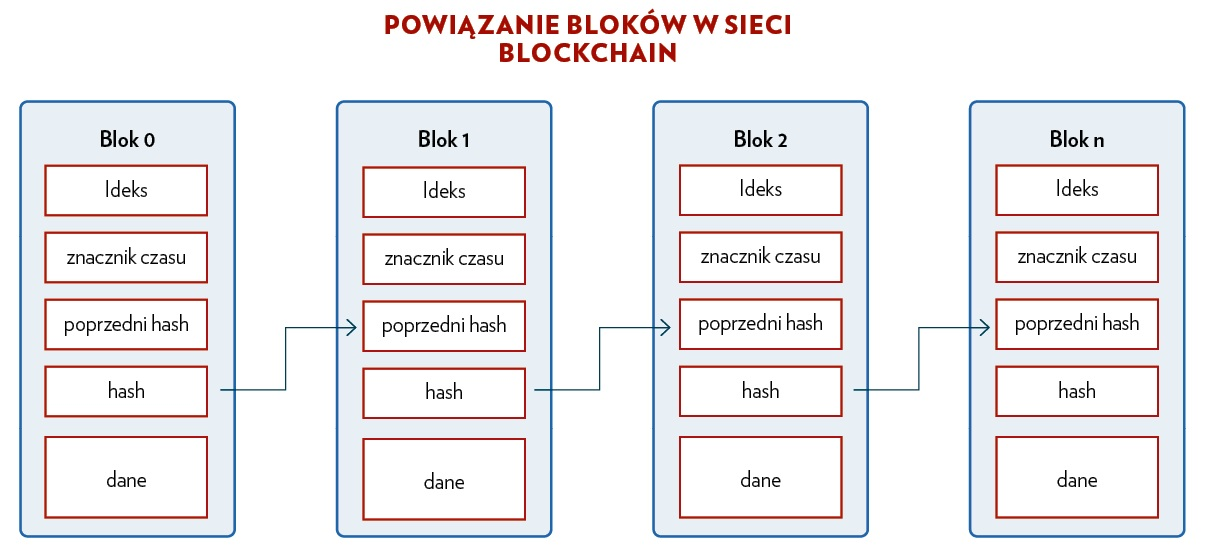
\includegraphics[width=\textwidth]{images/łańcuch_bloków.jpg}
	\caption {Łańcuch bloków.}
\end {figure}

Na rysunku 2.1 ukazany jest schemat łańcucha bloków. Jak widać dane przechowywane są w blokach, a bloki łączone są za pomocą wskaźników na hash poprzedniego bloku. Taka budowa stanowi zabezpieczenie łańcucha bloków przed modyfikacją lub usunięciem danych. Modyfikacja dowolnego bloku w sieci jest widoczna i łatwa do zweryfikowania. Wystarczy policzyć od początku hash dla każdego bloku i porównać z polem nastepnego bloku, które przechowuje poprzedni hash.

\subsection{Sieci Peer to Peer}

Zmodyfikowanie łańcucha bloków jest trudne, lecz nie jest niemożliwe. Wymaga jedynie wystarczająco dużej mocy obliczeniowej. Dodatkowo zamiast modyfikować łańcuch, można przejąć urządzenie, na którym uruchmomiony jest łańcuch bloków, co daje możliwość zakłócenia pracy systemu opartego na działaniu łańcucha.

Twórcy Bitcoina rozwiązali podane problemy wykorzystując zdecentralizowaną sieć Peer-to-Peer. Sieć Peer-to-Peer składa się z węzłów, które komunikują się ze sobą, bez centralnego serwera. Jeżeli węzły chcą się ze sobą skontaktować, to wysylają dane bezpośrednio do siebie. Takie rozwiązanie pozwala zwiększyć bezpieczeństwo sieci, ponieważ trudniej jest przejąć kontrole nad wieloma maszynami tworzącymi całą sieć, niż nad centalnym systemem obsługującym działanie tej sieci. Dodatkowo P2P zapewnia zabezpieczenie danych zgromadzonych w sieci, przed usunięciem, ponieważ każde urządzenie przechowuje swoje egzemplarze danych, które można traktować jako kopie zapasowe. Dystrybucja sieci na całym świecie zabezpiecza sieć przed ocenzurowaniem, z czego korzysta Bitcoin i inne kryptowaluty.

Peer-to-Peer jest przykładem ciekawego zastosowania architektury klient-serwer. Architektura klient serwer polega na podzieleniu systemu na stronę kliencką, która zajmuje się wysłaniem żądań do serwera, oraz na stronę serwerową, której zadaniem jest odpowiadanie na żądania, przechowywanie danych i operowanie na tych danych. W sieci P2P węzeł pełni role zarówno serwera, jak i klienta. Przykładowo węzeł może żądać przesłania danych od innego węzła, a także odpowiedzieć na żądanie innego węzła.

\subsection{Konsensus}

Konsensus w sieci Blockchain oznacza, że każdy z jej uczestników zgadza się na stan danych przechowywanych w sieci. Każda aktywność zmieniająca stan przechowywanych danych powinna być autoryzowana, aby zapewnić bezpieczeństwo i spójność sieci. Konsensus pozwala na wprowadzenie do sieci zestawu reguł, według których działa cała sieć. Takie działanie pozwala na zweryfikowanie zaufanego źródła i wykluczenie wpływu węzłów dziłających na szkodę sieci. W kryptowalutach najczęściej wykorzystywane algorytmy konsensusu to Proof of Work i Proof of Stake. Natommiast Proof of Authority dotyczy rozwiązań prywatnych.

\subsubsection{Proof of Work}

Proof of work to popularny w kryptowalucie Bitcoin algorytm uzyskiwania konsensusu. Algorytm ten wykorzystywany jest podczas tworzenia nowego bloku. Nowy blok wysyłany jest do wszystkich węzłów w sieci, które w celu dodania bloku do swojego łańcucha muszą zostać zatwierdzone. Na tym etapie algorytmu mamy do czynienia z popularnymi "koparkami" Bitcoinów. Aby blok został zatwierdzony węzeł musi wykonać pracę, czyli dokonać wkładu mocy obliczeniowej. Moc obliczeniowa wykorzystywana jest do rozwiązania zagadki matematycznej. Praca ta wykonywana jest przez węzeł i jest określana jako mining (pol. wydobywanie).Ten węzeł, który jako pierwszy rozwiąże zagadke, otrzyma nagrodę w postaci określonej ilości środków, w kryptowalucie Bitcoin. W typowych rozwiązaniach dla Bitocoinu poziom trudności dodania nowego bloku jest tak skonstruowany, aby nowe bloki były dodawane, w odstępach około 10 minutowych\cite{pow-bitcoin}. 

Takie rozwiązanie premiuje węzły, o większej mocy obliczeniowej. Dlatego w celu utrzymania spójności danych należy przeprowadzać synchronizację węzłów. Synchronizacja przebiega nastepująco: każdy węzeł rozsyła do całej sieci swój łańcuch, węzły porównują długość swojego łańcucha z nadesłanym łańcuchem i w węźle zapisywany jest dłuższy łańcuch. 

Proof of work to rozwiązanie towarzyszące architekturze Blockchain, od momentu jej powstania. Bitcoin poza dokonywaniem transakcji, pozwala na zarabianie poprzez tworzenie tzw. węzłów górniczych. Węzeł górniczy zajmuje się realizacją algorytmu Proof of Work, co oznacza rozwiązywanie zagadki matematycznej. Fizycznie jest to urządzenie, ze specjalistycznymi podzespołami i oprogramowaniem, które pozwala na uzyskanie wysokiej efektywności w wydobywaniu Bitcoina \cite{nodes}. Głównym problemem tego rozwiązania jest zużycie energii elektrycznej. W roku 2017 zużycie energii elektrycznej, przez wydobywanie Bitcoina było większe, niż w 159 krajach na świecie \cite{elctricity-bitcoin}. W 2019 naukowcy z University of Cambridge stworzyli specjalny indeks (CBECI), ukazujący dane dotyczące zużycia energii elektrycznej, przez Bitcoin'a \cite{CBECI}.

W tym algorytmie czynnik wkładu fizycznych zasobów, jest głównym motywatorem do uczciwego postępowania. Jednakże głownym czynnikiem sprawiającym, że ten algorytm działa jest pewność, że ponad 50\% uczestników sieci działa uczciwie. Ogrom inwestowanych zasobów wpływa na bezpieczeństwo sieci. Duża zdecentralizowana sieć Blockchain dysponuje ogromną mocą obliczeniową, na jej moc składa się moc wszystkich węzłów w sieci. Węzły różnią się mocą obliczeniową, natomiast decentralizacja sieci sprawia, że żaden z węzłów nie może przejąć kontroli nad całą siecią. Im większa decentralizacja tym bardziej zmniejsza się wpływ pojedynczego węzła na całą sieć. Co innego, gdy do sieci dołączona zostanie grupa węzłów, które będą stanowiły 51\% mocy obliczeniowej sieci oraz będą ze sobą współpracowały, działając na szkodę sieci. Taki scenariusz nazywany jest atakiem 51\%. Dysponując 51\% mocy obliczeniowej sieci, można bez wiedzy uczciwych uczestników, w szybszy sposób dodawać nowe bloki, co prowadzi do przejęcia obsługi dodawania zawartości, przez szkodliwych uczestników siec\cite{atack51}i.

W przypadku algorytmu Proof of Work atak 51\% jest bardzo rzadkim zjawiskiem, gdyż jest on bardzo drogi. Atak ten może być opłacalny jedynie wtedy, gdy atakujący chce zdestabilizować sieć. W przypadku Bitcoin'a destabilizacja sieci nie ma większego sensu, ponieważ dysponując taką mocą obliczeniową można uzyskać ogromne przychody z kopania Bitcoin'a, dodatkowo uzyskanie takiej mocy obliczeniowej w rozrastających się sieciach Blockchain dla Bitcoin'u jest na tyle drogie, że w teorii jest uznawane za nieosiągalne. Z tego powodu, w przypadku sieci Blockchain, bardzo ważne jest zadbanie o jak największe rozproszenie węzłów w sieci P2P.

\subsubsection{Proof of Stake}

Proof of Stake to kolejny algorytm używany do osiągania konsensusu w sieciach Blockchain. Jego największe zalety, to rozwiązanie problemu zużywania ogromnych ilości zasobów energii elektrycznej przez algorytm Proof of Work.

Działanie algorytmu Proof of Stake polega na wybieraniu spośród dostępnych węzłów sieci Blockchain walidatora. Walidator to węzeł, którego zadaniem jest weryfikacja poprawności bloku dołączanego do łańcucha. Wybór walidatora może się odbywać na różne sposoby, od całkowicie losowego wyboru, po wybór z uwzględnieniem czynników takich jak np. wiek stawki węzła, wysokość stawki. Stawka to zablokowane na koncie danego węzła jednostki waluty (kryptowaluty). Stawka jest wymagana, aby węzeł mógł uczestniczyć w losowaniu.

W przypadku algorytmu Proof of Stake głównym motywatorem uczciwego uczestnictwa w sieci jest możliwość utracenia części stawki. W przypadku wykrycia przez sieć nieprawidłowości w bloku dodanym przez konkretny węzeł, traci on określoną część stawki.

Proof of Stake jest o wiele bardziej ekologiczny, jeśli chodzi o zużycie energii elektrycznej, niż Proof of Work. Oznacza to, że sieć jest dostępna dla większej ilości urządzeń, co wpływa na zwiększenie rozproszenia sieci. W Proof of Stake głównym czynnikiem determinującym moc sieci jest zgromadzony w niej wkład finansowy w postaci stawek. W przypadku tego algorytmu również występuje problem ataku 51\%, jednakże tym razem atakujący musi dysponować odpowiednią ilością środków płatniczych, a dokładnie musi włożyć  51\% ogólnej stawki, co w przypadku Bitcoin'a jest mało prawdopodobne.

\subsubsection{Proof of Authority}
Proof of Authority to rozwiązanie skłaniające się ku mniej zdecentralizowanym systemom, które są tworzone na prywatne potrzeby i wymagających dużej przepustowości. Proof of Authority jest w swoim działaniu nieco zbliżony do Proof of Stake. Zamiast stawki podanej w jednostkach odpowiedniej waluty, w PoA używana jest reputacja walidatora. Prowadzi to do skonstruowania sieci, w której uczestniczą tylko zaufani walidatorzy. Uzyskanie statusu walidatora wiąże się z dużym nakładem pracy, w celu spełnienia kryteriów i uzyskania odpowiednio wysokiej reputacji. Podczas projektowania takiego systemu należy zwrócić szczególna uwagę, na stworzenie kryteriów o wysokiej trudności do spełnienia, aby wykluczyć węzły o szkodliwym działaniu.

Trudność uzyskania statusu walidatora bardzo mocno wpływa na stopień zdecentralizowania. Decentralizacja porównywalna z rozwiązaniem Proof of Stake jest niemożliwa do osiągnięcia.
Niski stopień decentralizacji wymaga pełnego zaufania do walidatorów, co może stanowić słaby punkt systemu, gdy zaufany waliadator zostanie przekupiony i dokona szkodliwej manipulacji na zawartości systemu.

Algorytm Proof of Authority świetnie sprawdza się w prywatnych sieciach Blockchain, gdy ważna jest wysoka przepustowość łącza. Jednakże należy pamiętać o odpowiednim doborze walidatorów.

\subsection{Funkcja skrótu}

Funkcje skrótu w systemach informatycznych pełnią rolę zabezpieczenia integralności danych. Zabezpieczenie danych polega na wykryciu modyfikacji. Matematyczna definicja funkcji skrótu h to odwzorowanie wiadomości m o dowolnej , skończonej długości, w ciąg bitów o określonej, stałej długości n \cite{hash}:

\begin{equation}
h:\left \{0, 1\right \}^{*}\rightarrow \left \{0, 1\right \}^{n}, gdzie: \left \{0, 1\right \}^{*}=\bigcup_{i\in  N}\left \{0, 1\right \}^{i}, N = \left \{0, 1, ...\right \}, n \in N
\end{equation}

Funkcja skrótu (hash) cechuje się wysoką podatnością na zmiany. Zmiana jednego bitu w danych wejściowych powoduje otrzymanie zupełnie innych wyników. \newline 
Przykładowo dla ciągu znaków hash0, dla funkcji skrótu SHA256 wynikiem jest ciąg znaków 
\newline 6ac73742db534bebccc9af1453c5637ee5bb5d7c9628ec2f26cf9777c89e96d8. Natomiast zmieniając ciąg znaków na hash1, otrzymanym wynikiem jest \newline af316ecb91a8ee7ae99210702b2d4758f30cdde3bf61e3d8e787d74681f90a6. Przykład obrazuje jak na wynikowy ciąg znaków wpływa zmiana jednego symbolu na wejściu.

Głównymi cechami funkcji skrótu są:
\begin{itemize}
	\item Nieodwracalność - na podstawie otrzymanego wyniku nie można bezpośrednio odtworzyć danych.
	\item Bezkolizyjność - nie istnieją dwa różne ciągi znaków, które dają ten sam wynik.
\end{itemize}

Znalezienie danych wejściowych dla funckji skrótu jest zadaniem wymagającym dużego nakładu mocy obliczeniowej. Dane można uzyskać losując wejściowy ciąg znaków i hashując go, a nastepnie porównując otrzymany hash z hashem, który ma być rozszyfrowany. Jest to tak zwany atak brutalny (ang. brute force).

Popularnym zastosowaniem funkcji skrótu jest podopis cyfrowy. Podpis cyfrowy to zaszyfrowany hash, wygenerowany na podstawie danych potrzebnych do podpisu. Głównym zaletą wykorzystania hash'owania w podpisie cyfrowym jest szybkość. Hashowanie wiadomości jest szybsze od szyfrowania, a zaszyfrować wystarczy sam ciąg znaków o stosunkowo małej długości, w porównaniu do tekstu wiadomości.

Funkcje skrótu można spotkać w bazach danych. Hasła są przykładem informacji, które w bazie danych są przechowywane w postaci funkcji skrótu. Takie rozwiązanie zabezpiecza hasła, w przypadku wycieku danych.

\subsection{Smart kontrakty.}

Wraz z powstaniem kryptowaluty Ethereum do architektury Blockchain została dodana nowa funkcja. Dodano tak zwane Smart Kontrakty

\newpage

\section{Technologia Blockchain na rynku.}

\subsection{Kryptowaluty.}

Kryptowaluta to cyfrowy środek płatniczy. W przeciwieństwie do tradycyjnych walut, kryptowaluty nie sa kontrolowane przez bank centralny. Środki płatnicze w kryptowalucie znajdują się w rozproszonej, po całym świecie sieci. Każda transakcja w tym środowisku jest zapisywana we współdzielonym rejestrze. Rejestr pozwala na ustalenie ile środków w danej kryptowalucie jest na koncie danego uczestnika sieci. Podstawą działania kryptowalut jest Blockchain. To Blockchain odpowiada za tworzenie rejestru transakcji, zabezpieczenie danych przed modyfikacją, współdzielenie danych i uzyskanie konsensusu. Przykładem takich kryptowalut są Bitcoin i Ethereum.

\subsection{Finanse.}

Dynamiczny rozwój technologii zapoczątkował rozwój innych branż, w tym sektora finansów. Powstała osobna gałąź tego sektora o nazwie FinTech. FinTech zajmuje się opracpwywaniem i wdrażaniem nowych technologii do systemów finansowych na całym świecie. Korzyści płynące z unowocześnienia sektora finansów mogą skupiają się głównie na zwiększeniu szybkości transakcji przez brak pośredników, zmniejszeniu kosztów przepływu transakcji i zwiększenie bezpieczeństwa. FinTech zajmuje się między innymi szukaniem zastosowań dla technologii Blockchain. Jako przykład rozwijania technologii blockchain przez FinTech może posłużyć przykład trwałego nośnika wdrożonego przez PKO Bank Polski. Trwały nośnik pozwala na dostarczanie klientom banku prywatnych dokumentów w formie cyfrowej \cite{PKO}. Twórcy tego rozwiązania zastoswali również mechanizm Smart Kontarktów. Smart Kontrakty są wykorzystywane do zautomatyzowania procesu egzekwowania umów ubezpieczeniowych\cite{PKO-SMART}. Pozwala to na zmniejeszenie uczestnictwa osób trzecich i redukcję kosztów.

\subsection{Internet of Things.}

Internet of Things to technologia pozwalająca na łączenie ze sobą wielu urządzeń. Tak skonstruowane sieci znajdują swoje przeznaczenie w systemach czasu rzeczywistego w przemyśle, bądź w inteligentnym domu. IoT wykorzystuje serwery internetowe, do przechowywania i pobierania danych. Blockchain w usługach IoT pomaga zabezpieczyć serwery z danymi, poprzez ich decentralizacje.

\newpage

\section{Przegląd istniejących rozwiązań e-votingu}
\section{System estoński}
Przykładem regularnego wykorzystania e-votingu jest Estonia. Estonia jest krajem, który pierwszy udostępnił możliwość głosowania elektronicznego w wyborach lokalnych, na szczeblu krajowym. W pierwszych wyborach wzięło udział około 1\% wyborców. Od roku 2005 w Estonii postępował rozwój systemów e-votingu. Wraz z następnymi wyborami zwiększała się liczba uczestników. W roku 2019 liczba wyborców, którzy skorzystali z e-votingu wyniosła 43,8\% wyborców.

Na system e-votingu  w Estonii składa się kilka mniejszych rozwiązań, które można wylistować w następujący sposób:
\begin{itemize}

    \item Identyfikacja za pomocą karty e-obywatela lub profilu e-obywatela w telefonie.

    \item Architektura rozwiązania pozwala na wysłanie wielu głosów, a głosem wiążącym jest zawsze głos finalny.

    \item Serwery wykorzystywane podczas głosowania są pod szczególną ochroną i nie można uzyskać do nich dostępu z bezpośrednio z internetu (zabezpieczenie firewallem).

    \item Wykorzystywanie prywatnych kluczy i narzędzi kryptograficznych w celu zabezpieczenia dostępu do danych. Wykorzystywanie standardu SSL.
    
\end{itemize}

\subsection{Przegląd rozwiązania}
Przebieg całego procesu wyborczego w Estonii można podzielić na kilka etapów:
\begin{itemize}
    \item ogłoszenie wyborów;
    \item zarejestrowanie kandydatów;
    \item przygotowanie list wyborczych;
    \item głosowanie;
    \item liczenie głosów;
    \item ogłoszenie wyników;
\end{itemize}

Wsparcie e-votingu (w Estonii określanego i-votingiem) obejmuje ostatnie trzy etapy procesu wyborczego.

\begin{figure}[h]
    	\centering
	\includegraphics[width=\textwidth]{images/Dziedzina systemu estońskiego}
	\caption{Moduły systemu i-votingu.}
\end {figure}
\newpage

W skład systemu głosowania wchodzą bazy danych przechowujące:
\begin{itemize}
    \item listę osób uprawnionych do głosowania;
    \item listę okręgów wyborczych;
    \item listę kandydatów lub opcji wyborczych;
    \item listę e-wyborców (i-voters);
\end{itemize}

Dostarczenie odpowiednich danych do systemu pozwala na walidację wyborcy, zgłoszenie przez 
niego głosu oraz zapisanie wyborcy, w bazie danych odpowiedzialnej za przechowanie listy e-wyborców. W skład logiki systemu wchodzą mechanizmy generujące wyniki. Wyniki e-votingu są scalane z wynikami wyborów tradycyjnych, przy czym scalanie nie pozwala na podwójne zliczenie głosu oddanego tradycyjnie i elektronicznie.

\begin{figure}[h]
    	\centering
	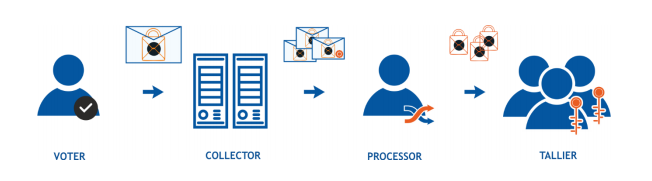
\includegraphics[width=\textwidth]{images/Główne częsci systemu estońskiego.png}
	\caption{Proces wyborczy.}
\end {figure}

Główne części systemu:
\begin{itemize}
    \item Voter (dalej nazywany wyborcą) - za pośrednictwem aplikacji klienckiej (która w systemie estońskim jest aplikacją desktopową pobieraną przed wyborami) szyfruje i zatwierdza swoim podpisem elektronicznym głos, który następnie wysyłany jest do Kolektora.
    \item Collector (dalej nazywany Kolektorem) - to aplikacja serwerowa wyposażona w logikę pozwalającą na utworzenie głosu. Aplikacja waliduje dane wprowadzone przez wyborce i elektronicznie podpisuje dane, które następnie przesyła do Procesora.
    \item Processor (dalej nazywany Procesorem) - zajmuje się przetwarzaniem głosów. Sprawdza poprawność danych otrzymanych z Kolektora, wraz z podpisem elektronicznym. Usuwa głosy, które się powtarzają, zarówno głosy oddane elektronicznie, jak i te oddane w lokalach wyborczych. Sortuje głosy według okręgów wyborczych i usuwa z nich podpis elektroniczny, w celu anonimizacji głosu. Tak przetworzone głosy są mieszane według odpowiedniego algorytmu i wysyłane do Licznika.
    \item Tallier (dalej nazywany Licznikiem) - rolą licznika jest odebranie głosu od Procesora, otwarcie go i dodanie przyporządkowanie do odpowiedniego wyniku.
\end{itemize}
\chapter{Projekt systemu}
System został zaprojektowany od strony teoretycznej, co oznacza wyszczególnienie modułów systemu, aktorów, przypadków użycia, modelów baz danych i wykorzystanych technologii. Obecny rozdział zawiera przegląd opracowanego rozwiązania oraz jego teoretyczny opis.

\section{Diagram przypadków użycia.}

W systemie można wyróżnić dwóch aktorów: wyborcę i administratora wyborów. Wyborca posiada funkcje typowe dla użytkownika serwisu internetowego. Posiada swoje konto, które po zalogowaniu udostępnia mu jako główną funkcję systemu, czyli możliwość oddania głosu. W celu oddania głosu użytkownik musi wybrać odpowiednie głosowanie, które jest dostarczane za pomocą API. Użytkownik może być przypisany do kilku trwających, bądź zaplanowanych głosowań. Po wyborze głosowania wyborca musi wybrać, na którego kandydata będzie głosował. Po wybraniu odpowiedniej kandydatury, wyborca wysyła swój głos. Wysłanie głosu jest równoznaczne z zakończeniem procesu głosowania. Dla każdego głosowania wyborca może wysłać tylko jeden głos, na jednego kandydata. Po wysłaniu głosów, użytkownik może się wylogować. W przypadku problemów z przejściem przez proces wyborczy, użytkownik może przeczytać instrukcję obsługi, która zawiera informacje o kolejnych krokach procesu wyborczego. Dodatkowo użytkownik może przeglądać wyniki wyborów, w których brał udział.

\begin{figure}[h]
    \centering
    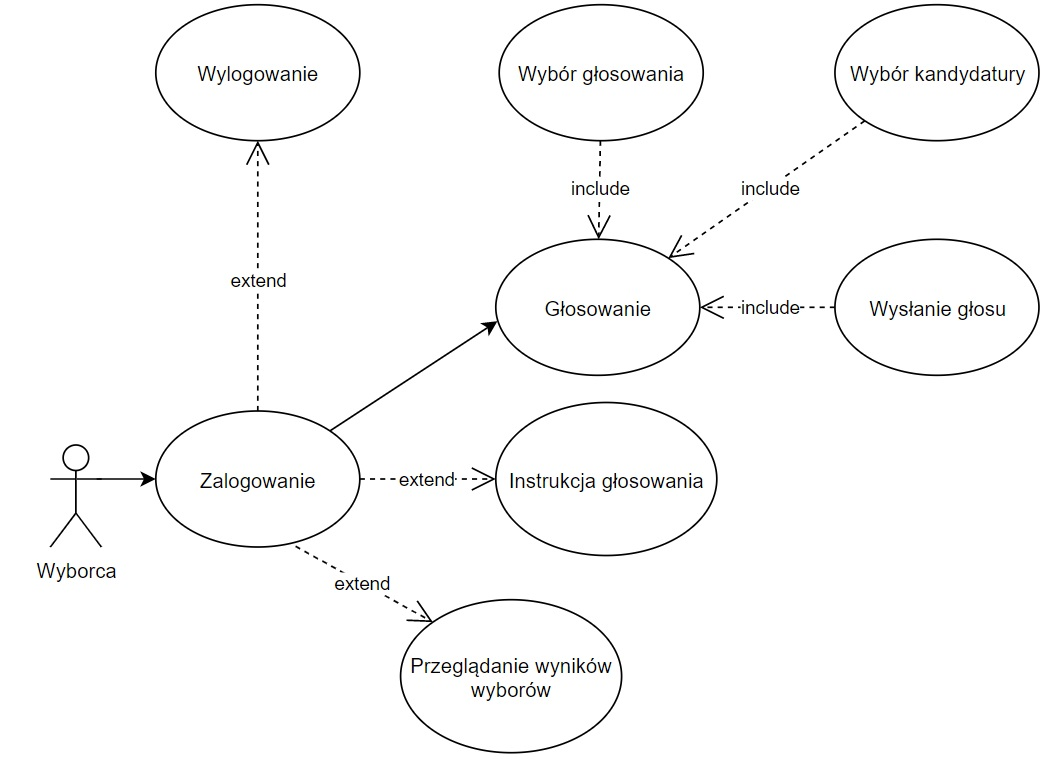
\includegraphics[scale=0.4]{images/user_use_case.jpg}
    \caption{Diagram przypadków użycia dla wyborcy.}
\end{figure}

\newpage

Administrator wyborów również posiada swoje konto, dzięki któremu musi się zalogować, aby mieć możliwość korzystania ze swoich funkcji. Głównym zadaniem administratora jest stworzenie wyborów. Tworzenie wyborów to proces odbywający się w kilu krokach. Pierwszym krokiem jest podanie odpowiedniego tytułu wyborów, opisu, daty rozpoczęcia i zakończenia oraz przypisania adresu serwera bazy danych, która przechowuje głosy. Etap ten jest określany jako konfiguracja wyborów. Następnym krokiem jest dodanie odpowiednich kandydatów oraz krótkich opisów. Ostatnim krokiem jest przypisanie wyborców dostępnych w bazie danych, dla których będą udostępnione wybory. Tak utworzone i skonfigurowane wybory, są dodawane do bazy danych.
Baza danych przechowująca konta wyborców może być w dowolnym momencie modyfikowana, poprzez stworzenie nowego konta wyborcy, bądź jego usunięcie. Administrator może również w niewielkim stopniu modyfikować trwające wybory, poprzez przypisanie nowego wyborcy i zmianę serwera bazy danych przechowującej głosy, w przypadku awarii. Jednym z najważniejszych zadań administratora jest ogłoszenie wyników wyborów. Po ogłoszeniu wyników wyborów, nie można dodawać głosów, a wyniki wyborów są udostępniane wyborcom.

\begin{figure}[h]
    \centering
    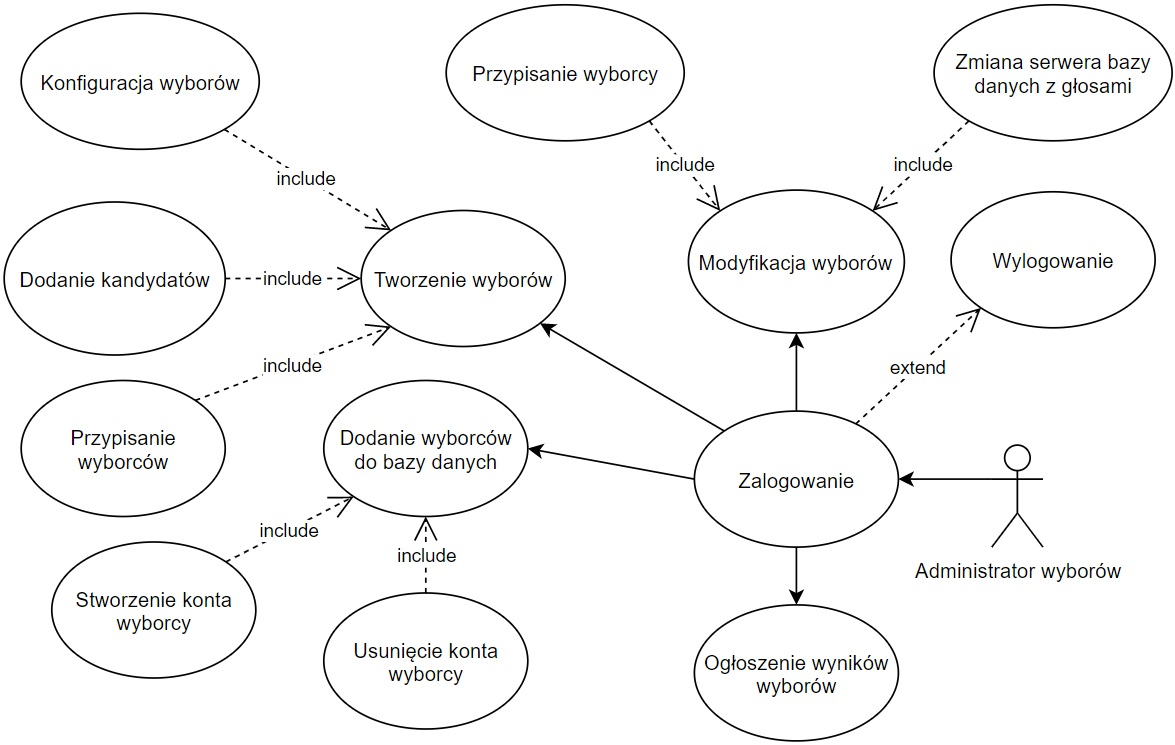
\includegraphics[scale=0.4]{images/admin_use_case.jpg}
    \caption{Diagram przypadków użycia dla administratora wyborów.}
\end{figure}

\newpage

\section{Podział systemu na moduły.}
System można podzielić na 4 moduły, które wchodzące ze sobą w interakcje tworzą spójną i działającą aplikację. Do tych modułów należą:
\begin{itemize}
    \item Serwer udostępniający API oraz baza danych.
    \item Aplikacja webowa wyborcy.
    \item Aplikacja webowa administratora.
    \item Sieci Blockchain, przechowujące głosy, tworzone są indywidualnie dla każdego głosowania.
\end{itemize}

\begin{figure}[h]
    \centering
    \includegraphics[scale=0.4]{images/moduły_systemu.jpg}
    \caption{Schemat przedstawiający moduły systemu.}
\end{figure}

\newpage

\section{API.}

Elementem centralnym całego systemu jest serwer dostarczający REST-API. API komunikuje się z wewnętrzną bazą danych, oraz zewnętrznymi sieciami Blockchain. Za pomocą otawartych endpointów serwera, użytkownicy i administratorzy mają dostęp do zasobów systemu. Dostep do zasobów jest zabezpieczony, za pomocą ról. W systemie występują dwie role: wyborca i administrator, podczas  żądania dostępu do danego zasobu użytkownik musi udowodnić przynależność do swojej roli. Określenie przynależności do roli znajduje się w bazie danych systemu. Za pośrednictwem serwera można uzyskać dostęp do dowolnego serwera pracującego w sieci Blockchain. Pozwala to na pobieranie informacji, audytowanie i konfigurowanie systemu.

Funkcjami serwera z REST-API są:
\begin{itemize}
	\item Obsługa komunikacji z bazą danych, rozumiana jako pobiernie, dodawanie, aktualizowanie i usuwanie danych.
	\item Komunkacja z sieciami Blockchain.
	\item Dostarczanie odpowiednich zasobów bazy danych użytkownikom, za pośrednictwem tzw. endpointów.
	\item Zabezpieczenie zasobów, przed nieuprawnionym dostępem. Uwierzytelnienie, w oparciu o role w systemie.
\end{itemize}

\section{Baza danych.}
Baza danych jest elementem ściśle powiązanym z API, dlatego API i baza danych są traktowane jako jeden moduł. Baza danych jest odpowiedzialna za przechowanie konfiguracji wyborów. Struktura bazy danych składa się z pięciu encji. Przedstawiona poniżej baza danych jest rozwiązaniem proponowanym, które zostało użyte podczas implementacji systemu.

\begin{figure}[h]
    \centering
    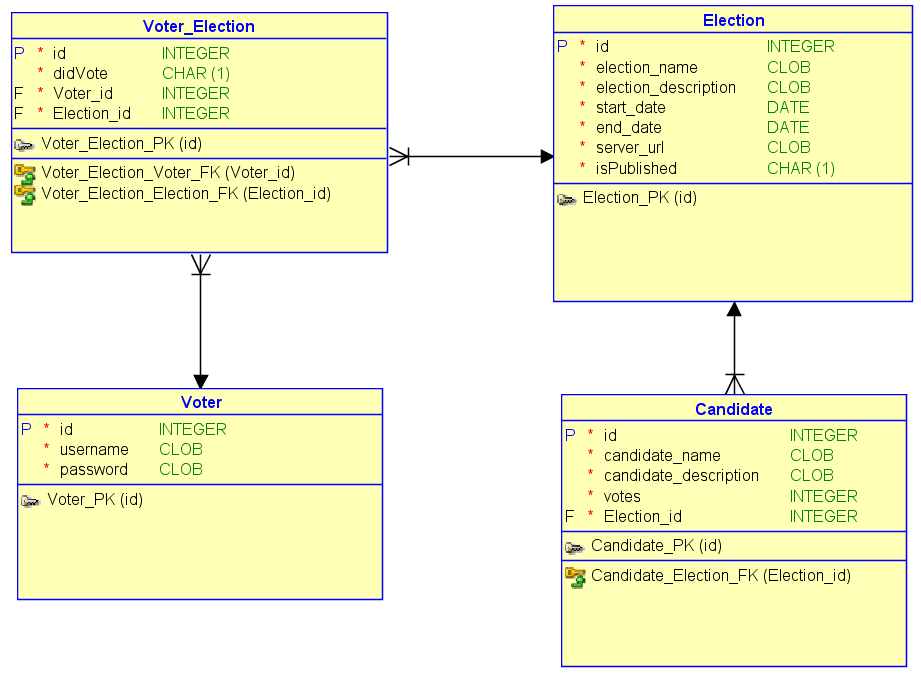
\includegraphics[scale=0.4]{images/Relational.png}
    \caption{Model fizyczny bazy danych}
\end{figure}

Encja Voter odpowiada profilowi wyborcy i przechowuje dane dotyczące logowania wyborców. Natomiast encja Election zajmuje się przechowaniem konfiguracji wyborów. Konfiguracji podlegają takie właściwości jak:
\begin{itemize}
	\item Tytuł wyborów (electionname).
	\item Opis dotyczący wyborów (electiondescription).
	\item Data rozpoczęcia  i zakończenia wyborów (startdate, enddate).
	\item Adres serwera sieci Blockchain, która jest odpowiedzialna za zbieranie głosów.
	\item Pole ispublished służy do poinformowania, o statusie danych wyborów. Gdy pole ma wartość 1, to wyniki wyborów są publiczne i wyborca ma do nich dostęp. W przeciwnym wypadku wyniki nie są dostępne dla wyborcy i czekaja na opublikowanie, przez administratora.
\end{itemize}

Encja o nazwie VoterElection, to tzw. encja łącznikowa, która ustanawia relacja wiele do wielu pomiędzy encjami Voter i Election. Dodatkowo przechowuje informację o oddaniu głosu w danych wyborach przez określonego użytkownika (atrybut didVote). 

Encja Candidate służy do reprezentacji kandydatów. 

Do funkcji bazy danych należą:
\begin{itemize}
    \item Przechowywanie danych logowania użytkowników i informacji o ich rolach.
    \item Uporządkowanie dostępu użytkowników do konkretnych wyborów.
    \item Przyporządkowanie kandydatów do wyborów i serializacja wyników.
    \item Baza danych dostarcza również strukturę, dzięki której można szybko dodawać nowe konfiguracje.
\end{itemize}

\section {Sieci Blockchain.}

Sieci Blockchain odpowiadają za przechowywanie głosów, dla określonych wyborów. Głównym argumentem za wykorzystaniem technologii Blockchain, w celu przechowania głosów, jest odporność na podmianę danych. Każda sieć odpowiada za jeden proces wyborczy. Sieć tworzona jest w opraciu o architekture Peer-to-Peer, co pozwala na rozproszenie węzłów.  Każdy węzeł to fizycznie serwer, posiadający uruchomione odpowiednie oprogramowanie. Oprogramowanie jest odpowiedzialne za dodawanie nowych bloków do łańcucha, synchronizację łańcuchów i utrzymanie konsensusu w sieci. 

Ważnym aspektem projektu jest wybór odpowiedniego algorytmu konsensusu. 

Dobór algoytmu konsensusu jest dowolny dla każdej sieci, ponieważ system wymaga informacji o tylko jednym węźle. Węzeł taki można nazwać węzłem głównym sieci, którego cechą jest utrzymanie bezpośredniej komunikacji z API. Węzeł ten zajmuje się:
\begin{itemize}
	\item Odebraniem głosów, które są wysłane z serwera centralnego za pośrednictwem API.
	\item Dostarczenie głosu do każdego węzła w sieci.
	\item Wysłanie zawartości łańcucha bloków do serwera centralnego.
	\item Wykonaniem operacji typowych dla każdego węzła w sieci: tworzenie nowych bloków, utrzymanie konsensusu i synchronizacja łańcuchów.
\end{itemize}

\begin{thebibliography}{99}
\bibitem{pa} Ankit Patel:
\emph{English \TeX},
https://medium.com/@ankit\_233/history-of-the-blockchain-1991-38d6d4c3420c

\bibitem{bitcoin} Academy Binance: Czym jest Bitcoin?
\emph{Polski \TeX},
https://academy.binance.com/pl/articles/what-is-bitcoin\#what-is-bitcoin

\bibitem{business} Vadapalli, Ravindhar:
\emph{English \TeX},
BLOCKCHAIN FUNDAMENTALS TEXT BOOK Fundamentals of Blockchain s. 10

\bibitem{4-concepts} Vadapalli, Ravindhar:
\emph{English \TeX},
BLOCKCHAIN FUNDAMENTALS TEXT BOOK Fundamentals of Blockchain s. 19

\bibitem{bitcoin-vs-blockchain} Academy Binance: Jaka jest różnica między Blockchainem a Bitcoinem?
\emph{English \TeX},
https://academy.binance.com/pl/articles/difference-between-blockchain-and-bitcoin

\bibitem{hash} ZESZYTY NAUKOWE AKADEMII MARYNARKI WOJENNEJ
ROK LIV NR 2 (193) 2013  Przemysław Rodwald : KRYPTOGRAFICZNE FUNKCJE SKRÓTU
\emph{English \TeX},
 s. 92

\bibitem{pow-bitcoin} Andrew Tar: Proof-of-Work, Explained. 2018.
\emph{English \TeX},  https://cointelegraph.com/explained/proof-of-work-explained

\bibitem{elctricity-bitcoin} Bitcoin Mining. 2017. 
\emph{English \TeX}, https://powercompare.co.uk/bitcoin/

\bibitem{nodes} Academy Binance: Węzły (nodes) - czym są i jak działają?
\emph{Polski \TeX},https://academy.binance.com/pl/articles/what-are-nodes

\bibitem{CBECI} Cambridge Bitcoin Electricity Consumption Index
\emph{English \TeX},https://www.epe.admin.cam.ac.uk/cambridge-bitcoin-electricity-consumption-index-cbeci

\bibitem{atack51} Sarwar Sayeed and Hector Marco-Gisbert: Assessing Blockchain Consensus and Security Mechanisms against the 51\% Attack
\emph{English \TeX} https://www.mdpi.com/2076-3417/9/9/1788/htm

\bibitem{PKO} PKO BP wdraża nową wersję trwałego nośnika. To pierwsze takie rozwiązanie w Europie
\emph{English \TeX} https://fintek.pl/pko-bp-wdraza-nowa-wersje-trwalego-nosnika-to-pierwsze-takie-rozwiazanie-w-europie/

\bibitem{PKO-SMART}BLOCKCHAIN W PKO BANKU POLSKIM
\emph{English \TeX} https://fintech.pkobp.pl/blockchain-w-banku/

\end{thebibliography}



\end{document}
